\documentclass[tikz,border=8pt]{standalone}
\usepackage{amsmath}
\begin{document}
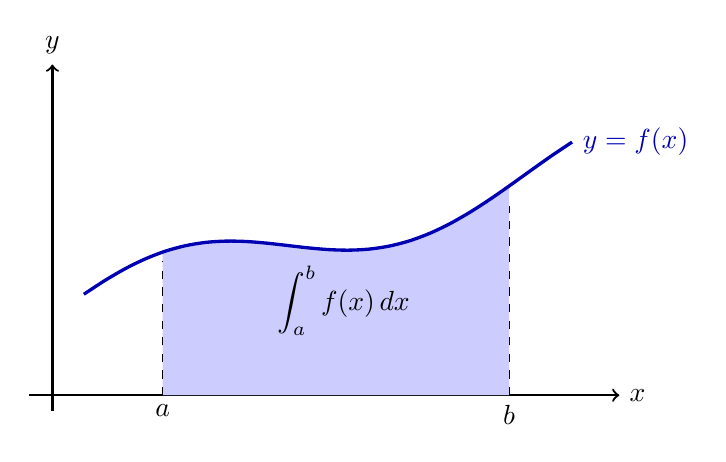
\begin{tikzpicture}
\draw[->, thick] (-0.3,0)--(7.2,0) node[right] {$x$};
\draw[->, thick] (0,-0.2)--(0,4.2) node[above] {$y$};
\fill[blue!20] (1.4,0)--plot[smooth,domain=1.4:5.8] (\x,{1+0.4*sin(60*\x)+0.3*\x})--(5.8,0)--cycle;
\draw[very thick,blue!70!black] plot[smooth,domain=0.4:6.6] (\x,{1+0.4*sin(60*\x)+0.3*\x}) node[right] {$y=f(x)$};
\draw[dashed] (1.4,0)--(1.4,1.7);
\draw[dashed] (5.8,0)--(5.8,2.4);
\node[below] at (1.4,0) {$a$}; \node[below] at (5.8,0) {$b$};
\node at (3.7,1.2) {$\displaystyle \int_a^b f(x)\,dx$};
\end{tikzpicture}
\end{document}